\chapter{Mathematical Model}
\label{chp:MAT}
%%%%%%%%%%%%%%%%%%%%%%%%%%%%%%%%%%%%%%%%%%%%%%%%%%%%%%%%%%%%%%%%%%%%%%%
We will apply quantitative methods in order to achieve the objectives listed. Since we intend to study the contribution of the birth dose and treatment of infected mothers to the transmission dynamics of the disease, we will employ population-based deterministic ordinary differential equations(ODE) models which we will adapt and modify from the existing literature. Population-based deterministic models are proper at this stage since we are only interested in how the infected population structure behaves when the suggested interventions are applied. Other tools which are appropriate in achieving the objectives could include: delay differential equation models so as to introduce a delay in terms of various events such as the kick-start of immunity, a delay in taking the routine vaccination, and so on, or partial differential equations so as to set up our model implicitly in terms of age and/or time. However, this is not the focus of our research question.

In applying the ODE models, our modelling process will take two ``stages":
In the first stage, we shall develop (or modify) several models from the literature. These models shall apply treatment independently to the infected mothers, and a combined strategy involving a birth dose alongside the routine vaccine to children. Here, the authors will assume that in reality, it will be done in primary health-care settings. These models will be simulated separately just as they have been described. Finally, we shall combine the two separate interventions we have described into a single model. A simulation of the three separate models over time will then produce outputs which will be fed into the second stage. 

On the matter of stage two, we will only be interested in the number of infants who remain infected after these interventions have been put in place. This output will flow into a larger SSA birth/death model for simulation over several generations.  
The total contribution of HBV+ children into the larger population will thus be the foundation
on which the hypothesis of eradication will be shown in this work.

\subsection{Mathematical Modeling}
We propose a mathematical model to study the long term contribution of the infected neonates to the general population-level infection dynamics. Our model studies the  impact of the administration of a birth and routine vaccine to infants, as well as treatment to infected pregnant women in sub-Saharan Africa where HBV is highly endemic.  

In our model, we assume that all infants take their first dose within 24 hours and the full routine vaccination within the next 6 months. This model serves as a feeder into a larger population model. It will feed the number of infants who remain infected (acute and chronic),  after several iterations, into the population model we shall develop.

To the best of our knowledge, not many models which consolidate HBV vertical transmission and two stages of vaccination have been published. In particular, none has been published, which studies the long term impact of combining a birth dose vaccine and a routine vaccine in the same model. 

To answer our research questions, we modify the models by \cite{mann2011modelling_NewZealand,zou2010modeling} by amalgamating ideas from the models in those papers. Of particular interest is the age-structured model by \cite{mann2011modelling_NewZealand}. We adapt the equation set (1) in \cite{mann2011modelling_NewZealand} for infants aged $0-1.25$ years since it captures the age structure of the neonates we intend to study, and modify it by including an extra dose of vaccination denoting the routine vaccination. For sub-question \ref{sub question 2}, we assume that there are two types of immunity induced in the infants for each stage of vaccination: for the birth dose, the infants acquire a temporary immunity which wanes. However, they acquire long term immunity if they proceed to receive the routine vaccination. The work by \cite{mclean1994modelling} extrapolated the vaccine-induced immunity period to be an average of 22.2 years from data which was collected over a period of 7 years. This vaccine-induced immunity acquired by these infants, we assume, is comparable to that acquired by the carrier individuals who clear the infection. This assumption is in contradiction to that of the model of \cite{zou2010modeling}. Our assumption is, however, justifiable since we only intend to simulate our model over a number of generations which amounts to a time period less than the average vaccine-induced immunity duration. It is therefore safe to equate the two types of acquired immunities described in our model and classify those two groups of individuals into the same epidemiological group. Again, in agreement with \cite{zhang2012analysisHBVmodel}, we assume that all infants born infected will be classified as chronic carriers. Finally, in accordance with \cite{mann2011modelling_NewZealand}, our model assumes that HBV-related deaths in the birth cohort in totality are negligible.

\subsubsection{Model Framework}
The model flowchart in figure \ref{fig:flowchart} describes a modified SIR type model adopted from \cite{zou2010modeling}.

The model consists of the following class of individuals, all of whom are neonates within their first 24 hours of birth: susceptible individuals, $S,$ infants with temporary protection from receiving the birth vaccine, $V,$ exposed neonates, $E,$ a class of individuals who have progressed from being exposed to having acute infections, $I,$ the HBV carriers, $C,$ and those with full immunity, $R$ .

\subsubsection{Flowchart Description}
Neonates are either born susceptible or infected and that is how $S$ and $C$ are populated. We assume that all infected infants go directly into the carrier class. The number of infected infants born to infected mothers is controlled by the efficacy of the treatment administered to the mothers. The susceptible individuals receive their first dose immediately after birth, moving to $V$ with temporary immunity. We, again, assume infants who receive the birth dose cannot be infected until after the vaccine wanes. We only allow waning of the birth vaccine for infants who will not proceed to receive the routine vaccine. The infants who receive the routine vaccine after the birth vaccine will populate the $R$ compartment with full protection alongside those neonates who will clear their infection. The infants who do not receive the birth vaccine, but remain uninfected until they receive the routine vaccine in full dosage will move to $R$ as well. The rest of the susceptible individuals either remain susceptible or go through the stages of being exposed to the infection from their mothers, and then, proceeding to the acute stage, and finally, the carrier phase. These infection stages described are only as a result of perinatal transmission as we assume horizontal transition is negligible at that age. We also assume hepatitis B related death to be negligible and so, in all the classes, mortality is only through natural death. 
\clearpage 		
The model flow diagram is represented in Figure \ref{fig:flowchart}. 
\begin{figure}[h!]
	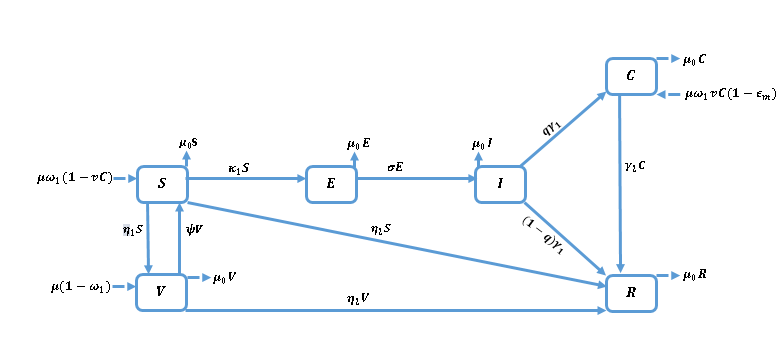
\includegraphics[scale=0.70]{infant_vaccination_model}
	\caption{the model structure indicating vertical transmission and two stages of immunity, the first through the birth vaccine, and final through a sort of booster by routine vaccination. The solid arrows indicate movement of the individuals, whiles the dashed arrows represent initial inflows and deaths.} \label{fig:flowchart}
\end{figure}

The systems of ordinary differential equations representing the dynamics described above are as follows:
\begin{align}
\begin{split}
\dfrac{dS}{dt}&=\mu\omega_1(1-\nu C)-(\mu_0+\kappa_1+\eta_2+\eta_1)S+\psi V\\
\dfrac{dV}{dt}&=\mu(1-\omega_1)+\eta_1S-(\mu_0+\eta_2+\psi)V \\
\dfrac{dE}{dt}&=\kappa_1S-(\mu_0+\sigma)E \label{eqn: 1}\\
\dfrac{dI}{dt}&=\sigma E-(\mu_0+\gamma_1)I\\
\dfrac{dC}{dt}&=(1-\epsilon_m)\mu\omega_1\nu C+q\gamma_1I-(\mu_0+\gamma_2)C\\
\dfrac{dR}{dt}&=\gamma_2C+(1-q)\gamma_1I+\eta_2(S+V)-\mu_0R
\end{split}
\end{align}
The various parameters used in our model are described the following table:

\vspace{1cm}
\begin{table}[t]
	\centering
	\begin{tabular}{ |p{1.57cm}|p{12cm}| }
		\hline
		Parameter& Description \\
		\hline
		$	\mu		$    	& 	birth rate    \\
		$	\mu_0 $			&  	natural death rate   \\
		$\kappa_1$ 			& 	MTCT transmission coefficient\\
		$\epsilon_m$ 		& 	efficacy of treatment of the infected mothers\\
		$\sigma$ 			& 	rate of progression from exposed state to acute state\\
		$\gamma_1$			& 	rate of moving from acute infection to carrier state\\
		$\gamma_2$ 			& 	rate of natural clearance of infection\\
		$\omega_1$			& 	proportion of infants without successful birth vaccination\\
		$\eta_1$ 			& 	birth vaccination rate\\
		$\eta_2$ 			&	routine vaccination rate\\
		$\psi$				&	waning rate of the birth vaccine\\
		$\nu$ 				& 	proportion of infants infected at birth\\
		$q$ 				& 	average probability that an infant proceeds to the carrier state due to inability to clear acute infection\\
		\hline
	\end{tabular}
	\caption{Model parameters and their descriptions}
	\label{table:1}
	
	
		\centering
		\begin{tabular}{ |p{1.57cm}|p{12cm}| }
			\hline
			Group & Description \\
			\hline
			$	S		$    		& 		Susceptible to the infection    \\
			$	V 		$			&  	 	Infants with the birth dose  	\\
			$	E 		$			&  	 	Exposed babies  				\\
			$	I 		$			&  	 	Acutely infected babies   		\\
			$	C       $ 			& 		HBV Chronic babies				\\
			$	R		$ 			& 		Fully immune individuals		\\
			\hline
		\end{tabular}
		\caption{Description of epidemiological grouping}
		\label{table:2}
		\vspace{1mm}
\end{table}
